\documentclass[pdf,xcolor={rgb},aspectratio=169]{beamer}
\usepackage[]{hyperref,graphicx,siunitx,lmodern,booktabs,tikz,pgfplots,pgfplotstable}
\usepackage{pdfpc-commands}

\usepackage[mode=buildnew]{standalone}
\mode<presentation>{\usetheme{Astro}}

\graphicspath{ {../Images/} }

\sisetup{per-mode=symbol}
\usetikzlibrary{calc,patterns, decorations.pathmorphing, fadings}
\pgfmathdeclarefunction{planck}{1}{\pgfmathparse{1.19E-16/x^5*1/(exp(0.0144/(x*#1))-1)}}
\pgfmathdeclarefunction{gauss}{3}{\pgfmathparse{#3*exp(-((x-#1)^2)/(2*#2^2))}}
\pgfdeclarehorizontalshading{rainbow}{100bp}{
  color(0bp)=(violet);
  color(30bp)=(black!30!violet); 
  color(38bp)=(blue);
  color(42bp)=(black!20!cyan);
  color(46bp)=(green); 
  color(52bp)=(yellow);
  color(58bp)=(orange);
  color(65bp)=(red); 
  color(73bp)=(black!60!red);
  color(100bp)=(black!50!red)
}

\newcommand{\linespectra}[2]{
  \coordinate (init) at (#1);
  \fill[shading=rainbow, opacity=0.1] (init) rectangle +(4,1);
  \foreach \f in {#2}{
	\definecolor{col}{wave}{\f}
	%\fill[left color=transparent,right color=transparent,middle color=col] ($(init)+(\f/100-4,0)$) rectangle +(0.5mm,1cm);
	\fill[col, path fading=east] ($(init)+(\f/100-3.5+0.025,0)$) rectangle +(0.25mm,1cm);
	\fill[col, path fading=west] ($(init)+(\f/100-3.5+0.025,0)$) rectangle +(-0.25mm,1cm);
	%\node[white,anchor=west,font=\tiny, rotate=-90] at ($(init)+(\f/100-4+0.025,0)$) {\f nm};
  \draw[black,very thick] (init) rectangle +(4,1);
  }
}

\newcommand{\absorbspectra}[2]{
  \coordinate (init) at (#1);
  \fill[shading=rainbow, opacity=0.8] (init) rectangle +(4,1);
  \draw[black,very thick] (init) rectangle +(4,1);
  \foreach \f in {#2}{
	\definecolor{col}{wave}{900}
	%\fill[left color=transparent,right color=transparent,middle color=col] ($(init)+(\f/100-4,0)$) rectangle +(0.5mm,1cm);
	\fill[col, path fading=east] ($(init)+(\f/100-3.5+0.025,0)$) rectangle +(0.25mm,1cm);
	\fill[col, path fading=west] ($(init)+(\f/100-3.5+0.025,0)$) rectangle +(-0.25mm,1cm);
	%\node[white,anchor=west,font=\tiny, rotate=-90] at ($(init)+(\f/100-4+0.025,0)$) {\f nm};
  }
}

%preamble
\title{A Seance with the Spectral}
\date{September 19, 2018}
\author{Jed Rembold}

\begin{document}
\renewcommand*{\theenumi}{\Alph{enumi}}

\begin{frame}{Announcements}
	\begin{itemize}
	  \item WebWorK due Friday
	  \item Test 1 is a week from Friday!
		\begin{itemize}
		  \item Old tests and review questions will be posted Friday so you can start studying
		  \item Lecture review questions and understanding checks also a good source to check yourself
		  \item I'm working to get the equation page updated and posted
		\end{itemize}
	\item Polling: \nolinkurl{rembold-class.ddns.net}
	\end{itemize}
\end{frame}

\begin{frame}{Review Question}
	Given the wave below, what is the wavelength of the wave? Each grid is 1 meter.
	\begin{enumerate}
		\item \SI{1}{\meter}
		\item \SI{1.5}{\meter}
		\item \alert<2>{\SI{3}{\meter}}
		\item \SI{10}{\meter}
	\end{enumerate}
	\begin{center}
		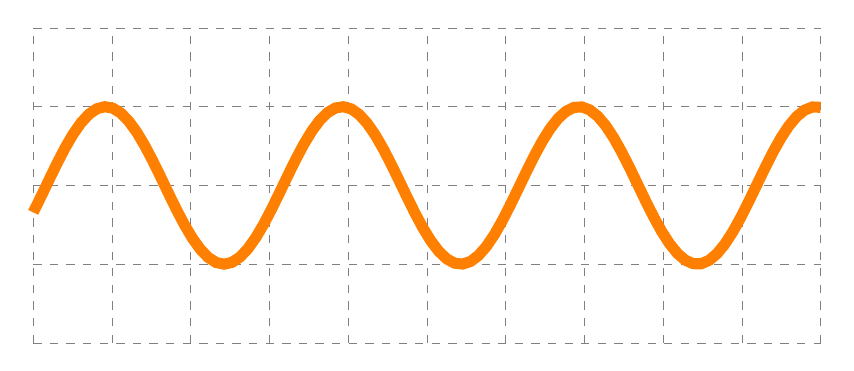
\begin{tikzpicture}
			\draw[help lines,dashed] (0,-2) grid (10,2);
			\draw[orange, line width=4pt, domain=0:10, samples=100] plot (\x,{sin(2.09*\x r - 20)});
		\end{tikzpicture}
	\end{center}
\end{frame}

%\begin{frame}{Review Question}
  %The plot below is a spectrum from a radiating blackbody. If the temperature of the blackbody was increased, the spectral peak would:
  %\begin{columns}
	%\column{.4\textwidth}
	%\begin{enumerate}
	  %\item \alert<2>{Get higher and move left}
	  %\item Get higher and move right
	  %\item Get lower and move left
	  %\item Get lower and move right
	%\end{enumerate}
	%\column{.5\textwidth}
	%\begin{center}
	  %\begin{tikzpicture}
		%\begin{axis}[width=6cm, height=6cm, samples=100,smooth, hide axis, ymin=0, xmin=0]
		  %%\addplot+[mark=none, orange, ultra thick, domain=0:5E-6] {1/x^5*1/(exp(0.0144/(x*4000))-1)};
		  %\addplot+[mark=none, orange, ultra thick, domain=0:5E-6] {planck(3000)};
		%\end{axis}
		%\draw[latex-latex] (5,0) -- node[midway,below] {Wavelength} (0,0) -- node[midway,sloped,above] {Energy Output} (0,4);
	  %\end{tikzpicture}
	%\end{center}
  %\end{columns}
%\end{frame}

\begin{frame}{I'm (Mostly) Blind!}
  \begin{center}
	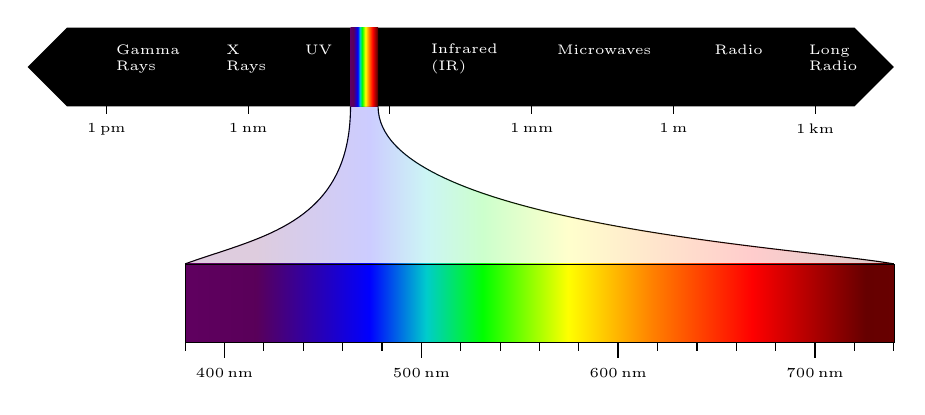
\begin{tikzpicture}
	  %Drawing the Bottom
	  \shade[shading=rainbow] (0,0) rectangle (9,1);
	  \draw[very thin] (0,0) rectangle (9,1);
	  \draw (0,0) -- (9,0);
	  \foreach \x in {0,0.5,...,9} \draw[thin] (\x,0) -- (\x,-0.1);
	  \foreach \x/\num in {0.5/400,3/500,5.5/600,8/700}{
		  \draw[semithick] (\x,0) -- (\x,-0.2)
			  node[below,font=\tiny] {$\SI{\num}{\nano\meter}$};
	  }

	  %Drawing the Top
	  \fill[black] (-1.5,3) -- (8.5,3) -- (9,3.5) -- (8.5,4) -- (-1.5,4) -- (-2,3.5) -- cycle;
	  \shade[shading=rainbow] (2.1,3) coordinate (x1) rectangle +(.35,1) coordinate (p2);
	  \foreach[count=\c] \x in {-1,0.8,...,8.1} \draw (\x,3) -- (\x,2.9) coordinate (\c);
	  \begin{scope}[font=\tiny, below]
		\node at (1) {$\SI{1}{\pico\meter}$};
		\node at (2) {$\SI{1}{\nano\meter}$};
		%\node at (3) {$\SI{1}{\micro\meter}$};
		\node at (4) {$\SI{1}{\milli\meter}$};
		\node at (5) {$\SI{1}{\meter}$};
		\node at (6) {$\SI{1}{\kilo\meter}$};
	  \end{scope}

	  \begin{scope}[right,font=\tiny,right,color=white, text width=1cm]
	  \node at (-1.0,3.6) {Gamma Rays};
	  \node at (0.4,3.6) {X Rays\phantom{gamma}};
	  \node at (1.4,3.6) {UV \phantom{gamma}};
	  \node at (3.0,3.6) {\centering Infrared (IR)};
	  \node at (4.6,3.6) {Microwaves \phantom{gamma}};
	  \node at (6.6,3.6) {Radio \phantom{gamma}};
	  \node at (7.8,3.6) {Long Radio\phantom{gamma}};
	  \end{scope}


	  %Connecting Bits
	  \draw[thin] (x1) ..controls +(-90:1.5) and +(20:1).. (0,1) coordinate(z1);
	  \draw[thin] ($(p2)-(0,1)$) coordinate (x2) ..controls +(-90:1.5) and +(170:1.2).. (9,1) coordinate(z2);
	  %Shading the Connecting Bits
	  \shade[shading=rainbow,opacity=0.2] (x1)..controls +(-90:1.5) and +(20:1).. (0,1) -- (9,1) ..controls +(170:1.2) and +(-90:1.5)..(x2)--cycle;
	\end{tikzpicture}
  \end{center}
  \tiny{Please just pause a moment and appreciate this lovely thing that I spend forever on\ldots}
\end{frame}

\fullFrameImageZoomedHorizontal{ch5_deepfield.jpg}

\begin{frame}{Everything the Light touches\ldots}
  \begin{itemize}
	\item Everything that emits or reflects light we can observe
	\item The visible bits are just a tiny fraction of the huge spectrum of possibilities
	\item Gives rise to different forms of astronomy:
	  \begin{itemize}
		\item Optical
		\item Radio
		\item Microwave
		\item High Energy (Gamma/X Ray)
	  \end{itemize}
  \end{itemize}
\end{frame}

\begin{frame}{Some more difficult than others\ldots}
  \begin{center}
	\includegraphics[width=\textwidth]{ch5_Atmosphere_Opacity.pdf}
  \end{center}
\end{frame}

%\begin{frame}{Light is Discrete}
  %\begin{itemize}
	%\item Why do the high energy type events correspond to lower wavelengths?
	%\item An issue with the wave theory of light:
	  %\begin{itemize}
		%\item Noticed some metals would give off electrons when light was shone on them
		%\item Oddly, the intensity (amplitude) of light didn't change the number of electrons
		%\item The wavelength (or frequency) of the light DID change the number
		%\item How to explain?
	  %\end{itemize}
  %\end{itemize}
%\end{frame}

%\begin{frame}{The Photoelectric Effect}
  %\begin{center}
	%\begin{tikzpicture}
	  %\fill[pattern=north east lines, pattern color=fg] (0,0) rectangle (8,-0.5);	  
	  %\draw[very thick] (0,0) -- (8,0);
	  %\draw[decorate, decoration={snake, segment length=5mm, amplitude=2mm}, ultra thick, red] (1,0) -- +(135:3);
	  %\draw[decorate, decoration={snake, segment length=3mm, amplitude=2mm}, ultra thick, green] (3,0) -- +(135:3);
	  %\draw[dashed, ultra thick, green] (3,0) -- node[midway,sloped,below] {fast}+(60:2) node[fill,circle,inner sep=0pt, minimum size=5pt] {};
	  %\draw[decorate, decoration={snake, segment length=2mm, amplitude=2mm}, ultra thick, violet] (7,0) -- +(135:3);
	  %\draw[dashed, ultra thick, violet] (7,0) -- node[midway,sloped,below] {faster}+(60:3) node[fill,circle,inner sep=0pt, minimum size=5pt] {};
	%\end{tikzpicture}
  %\end{center}
  %\begin{itemize}
	%\item Einstein found that light transfers energy in discrete chunks, called quanta
	%\item The energy in each quanta is related to the wavelength
	  %\begin{itemize}
		%\item Smaller wavelengths (higher frequency) = higher energy
	  %\end{itemize}
  %\end{itemize}
  %\begin{alertblock}{Light: Because life is complicated}
	%Light behaves both like a wave \emph{and} like a particle!
  %\end{alertblock}
%\end{frame}

\begin{frame}{Back to the Spectrum}
  \begin{center}
	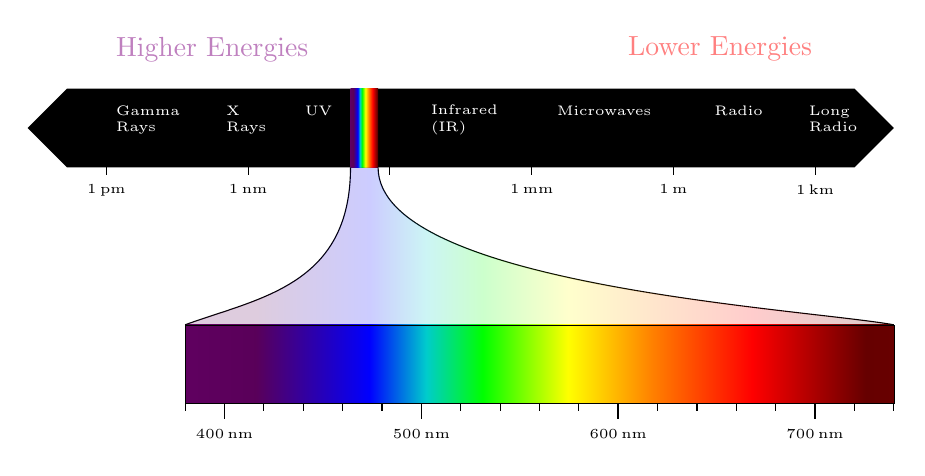
\begin{tikzpicture}
	  %Drawing the Bottom
	  \shade[shading=rainbow] (0,0) rectangle (9,1);
	  \draw[very thin] (0,0) rectangle (9,1);
	  \draw (0,0) -- (9,0);
	  \foreach \x in {0,0.5,...,9} \draw[thin] (\x,0) -- (\x,-0.1);
	  \foreach \x/\num in {0.5/400,3/500,5.5/600,8/700}{
		  \draw[semithick] (\x,0) -- (\x,-0.2)
			  node[below,font=\tiny] {$\SI{\num}{\nano\meter}$};
	  }

	  %Drawing the Top
	  \fill[black] (-1.5,3) -- (8.5,3) -- (9,3.5) -- (8.5,4) -- (-1.5,4) -- (-2,3.5) -- cycle;
	  \shade[shading=rainbow] (2.1,3) coordinate (x1) rectangle +(.35,1) coordinate (p2);
	  \foreach[count=\c] \x in {-1,0.8,...,8.1} \draw (\x,3) -- (\x,2.9) coordinate (\c);
	  \begin{scope}[font=\tiny, below]
		\node at (1) {$\SI{1}{\pico\meter}$};
		\node at (2) {$\SI{1}{\nano\meter}$};
		%\node at (3) {$\SI{1}{\micro\meter}$};
		\node at (4) {$\SI{1}{\milli\meter}$};
		\node at (5) {$\SI{1}{\meter}$};
		\node at (6) {$\SI{1}{\kilo\meter}$};
	  \end{scope}

	  \begin{scope}[right,font=\tiny,right,color=white, text width=1cm]
	  \node at (-1.0,3.6) {Gamma Rays};
	  \node at (0.4,3.6) {X Rays\phantom{gamma}};
	  \node at (1.4,3.6) {UV \phantom{gamma}};
	  \node at (3.0,3.6) {\centering Infrared (IR)};
	  \node at (4.6,3.6) {Microwaves \phantom{gamma}};
	  \node at (6.6,3.6) {Radio \phantom{gamma}};
	  \node at (7.8,3.6) {Long Radio\phantom{gamma}};
	  \end{scope}

	  \node[violet!50,anchor=west] at (-1,4.5) {Higher Energies};
	  \node[red!50,anchor=west] at (5.5,4.5) {Lower Energies};

	  %Connecting Bits
	  \draw[thin] (x1) ..controls +(-90:1.5) and +(20:1).. (0,1) coordinate(z1);
	  \draw[thin] ($(p2)-(0,1)$) coordinate (x2) ..controls +(-90:1.5) and +(170:1.2).. (9,1) coordinate(z2);
	  %Shading the Connecting Bits
	  \shade[shading=rainbow,opacity=0.2] (x1)..controls +(-90:1.5) and +(20:1).. (0,1) -- (9,1) ..controls +(170:1.2) and +(-90:1.5)..(x2)--cycle;
	\end{tikzpicture}
  \end{center}
\end{frame}

\begin{frame}{How to make some light\ldots}
  \begin{itemize}
	\item The general term \underline{electromagnetic radiation} describes all the frequencies, not just the visible ones we generally call ``light''
	\item How do we produce EM-radiation?
	  \begin{itemize}[<+->]
		\item Take something hot\ldots
		\item \ldots or warm \ldots
		\item \ldots or not 100\%, absolutely cold
	  \end{itemize}
	\item What wavelengths are emitted depend on the objects temperature
	  \begin{itemize}[<+->]
		\item Hot object produce more radiation in general
		\item Hot objects produce more radiation at shorter wavelengths
	  \end{itemize}
  \end{itemize}
\end{frame}

\begin{frame}{A shining example \footnotesize(ba-dump tssh)}
  \begin{columns}
	\column{.5\textwidth}
	\begin{itemize}
	  \item Star color depends on the star's temperature!
	  \item The brightness we see also depends on the star's size and distance from us (more on that later!)
	\end{itemize}
	\column{.5\textwidth}
	\begin{center}
	  \includegraphics[width=.7\textwidth]{ch5_orion.jpg}
	\end{center}
  \end{columns}
\end{frame}

\begin{frame}{Brighter and Bluer\ldots}
  \begin{itemize}
	\item So hotter objects radiate both
	  \begin{itemize}
		\item more total radiation and
		\item lower wavelength radiation
	  \end{itemize}
	\item Qualitatively this moves our spectrum to the left and makes it taller
	\item Quantitatively, we can describe this effect through two laws!
	  \begin{itemize}
		\item Stefan-Boltzmann Law
		\item Wien's Law
	  \end{itemize}
  \end{itemize}
  \begin{alertblock}{Important!}
	  Increasing an object'ss temperature causes it to emit light that is both bluer (of a lower average wavelength) and brighter (of a greater amplitude)
  \end{alertblock}
\end{frame}

%\begin{frame}{Stefan-Boltzmann Law}
  %\begin{itemize}
	%\item Hot objects emit more total radiation than cool objects
	  %\begin{itemize}
		%\item Aka, they are brighter
	  %\end{itemize}
	%\item \alert{Intensity} ($I$) of radiation is a measure of how much energy per second per area a radiator is outputting
	%\item Can think of as the area underneath our spectral curve
	%\item For blackbody radiation, $I$ depends only on the temperature!
	  %\[I = \sigma T^4\]
	%\item Here $\sigma$ is the Stefan-Boltzmann constant and equals:
	  %\[\sigma = \SI{5.67e-8}{\joule\per\square\meter\per\second\per\kelvin^4}\]
	%\item Note that this is why the SIZE of the object matters as well!
  %\end{itemize}
%\end{frame}

%\begin{frame}{Great Balls of Fire! (Or tiny ones\ldots)}
  %\begin{columns}
	%\column{.5\textwidth}
	  %\begin{example}
		%Suppose I take a superheated ball of nickel and set it onto a block of ice. How much energy is it radiating each second? Judging by the video, the nickel is maybe \SI{3}{\centi\meter} in diameter and glowing a whitish-yellow, which would correspond to a temperature of about \SI{4700}{\kelvin}.
	  %\end{example}
	%\column{.5\textwidth}
	%\inlineMovie{../Videos/Nickelball.ogv}{../Videos/Nickelball.jpg}{width=\textwidth}
  %\end{columns}
%\end{frame}

\begin{frame}{Wien's Law}
  \begin{itemize}
	\item Wien's Law tells us at what wavelength the \emph{peak} of the spectral curve lies.
	\item Thus it gives us information about the color
	\item Very simple relation:
	  \[\lambda_{max} (\si{\nano\meter}) \approx \frac{2900000}{T}\]
	\item \alert{Note that this equation gives you the wavelength in nanometers!}
  \end{itemize}
  \begin{center}
	\begin{tikzpicture}
	  \begin{axis}[domain=0:2000E-9,width=\textwidth, height=4cm, samples=50, smooth,xmin=0, scaled ticks=false, xtick={241e-9, 483E-9, 966E-9},xticklabels={\textcolor{cyan}{241}, \textcolor{yellow!50}{483}, \textcolor{red!50}{966}}, xlabel=Wavelength (nm), yticklabels={,,}]
		\addplot+[mark=none,ultra thick, cyan] {planck(12000)};
		\addplot+[mark=none,ultra thick, yellow!50] {20*planck(6000)};
		\addplot+[mark=none,ultra thick, red!50] {200*planck(3000)};
	  \end{axis}
	\end{tikzpicture}
  \end{center}
\end{frame}

\begin{frame}{Life is complicated}
  \begin{itemize}
	\item Unfortunately, not everything radiates as well as coals or stars
	\item How well an object radiates is called it's emissivity ($\varepsilon$)
  \end{itemize}
  \begin{center}
	\begin{tikzpicture}
	  \begin{axis}[domain=0:6000E-9,scaled ticks=false, samples=50, smooth,xmin=0,ymin=0, ticks=none,xlabel near ticks,ylabel near ticks,xlabel=Wavelength, ylabel=Energy Output,axis lines=left, axis line style={-latex}, height=7cm]
		\only<1->{\addplot+[mark=none,yellow, ultra thick] {planck(2000)} node[pos=.6,right] {$\varepsilon=1$};}
		\only<2->{\addplot+[mark=none,dashed,yellow!50, ultra thick] {.8*planck(2000)} node[pos=.7,left] {$\varepsilon=.8$};}
	  \end{axis}
	  \onslide<3->{\draw[ultra thick, green] (0,0) to[out=0, in=180] (2,2) to[out=0, in=180] (4,1) to[out=0, in=180] (6,5) node[right] {Not a blackbody!};}
	\end{tikzpicture}
  \end{center}
\end{frame}

\fullFrameImageZoomedHorizontal{ch5_sun_spectrum.jpg}

\begin{frame}{Spectra and Composition}
  \begin{itemize}
	\item Objects with thermal spectra are generally dense (wood, rocks, people, metals, stars,\ldots)
	\item A perfect ``blackbody'' spectrum would \emph{only} give us information about the temperature
	\item Diffuse gases have a more complex spectra, and indeed one that gives information about their chemical composition
	  \begin{itemize}[<2->]
		\item \alert{Why is gas so special?}
	  \end{itemize}
  \end{itemize}
\end{frame}

\begin{frame}{Life of an Electron}
  \begin{itemize}
	\item Electrons orbit around the nucleus of an atom
	\item<2-> Only allowed in certain areas $\rightarrow$ Energy levels
	\item<3-> Height of stairs determined by nucleus
  \end{itemize}
  \begin{center}
	\begin{tikzpicture}
	  \onslide<1>{
		\shade[inner color=yellow, outer color=Background] (0,0) circle (2cm);
		\fill[ball color=cyan] (1,0) circle(2pt);
	  }
	  \fill[ball color=red] (0,0) circle(3pt);
	  \onslide<2->{
		\draw[yellow] (2,-2) -- coordinate[midway] (e1) ++(1,0)-- ++(0,1)-- coordinate[midway] (e2) ++(1,0)--++(0,.5)-- coordinate[midway] (e3) ++(1,0)--++(0,.25)-- coordinate[midway] (e4) ++(1,0) coordinate (end);
		\draw[orange,latex-] ($(end)-(0,.25)$) --+(0,-1.5) node[midway,sloped,above] {Energy};
	  }
	  \onslide<2->{
		\draw[yellow,dashed] (0,0) circle(0.5cm);
		\draw[yellow,dashed] (0,0) circle(1cm);
		\draw[yellow,dashed] (0,0) circle(1.5cm);
		\draw[yellow,dashed] (0,0) circle(2cm);
	  }
	  \onslide<2,3>{
		%\fill[ball color=cyan] (e1) circle(2pt);
		\fill[ball color=cyan] (0.5,0) circle(2pt);
		\fill[ball color=cyan] (e1) circle(2pt);
	  }
	  \onslide<3>{
		\draw[green, thick, latex-, decorate, decoration={snake, pre length=1mm}] (0.5,0) --+(45:2);
	  }
	  \onslide<4>{
		\draw[cyan,-latex] (0.5,0) to[bend right] (1,0);
		\draw[cyan,-latex] (e1) to[bend right] (e2);
		\fill[ball color=cyan] (1,0) circle(2pt);
		\fill[ball color=cyan] (e2) circle(2pt);
	  }
	  \onslide<5>{
		\draw[red, thick, latex-, decorate, decoration={snake, pre length=1mm}] (1,0) --+(45:2);
		\fill[ball color=cyan] (1,0) circle(2pt);
		\fill[ball color=cyan] (e2) circle(2pt);
	  }

	  \onslide<6>{
		\draw[cyan,-latex] (1,0) to[bend right] (1.5,0);
		\draw[cyan,-latex] (e2) to[bend right] (e3);
		\fill[ball color=cyan] (e3) circle(2pt);
		\fill[ball color=cyan] (1.5,0) circle(2pt);
	  }
	  \onslide<7>{
		\draw[violet, thick, -latex, decorate, decoration={snake, post length=1mm}] (1.5,0) --+(45:2);
		\fill[ball color=cyan] (e1) circle(2pt);
		\fill[ball color=cyan] (0.5,0) circle(2pt);
		\draw[cyan,-latex] (1.5,0) to[bend left] (0.5,0);
		\draw[cyan,-latex] (e3) to[bend left] (e1);
	  }
	\end{tikzpicture}
  \end{center}
\end{frame}

\begin{frame}{Fingerprinting Light}
  \begin{itemize}
	\item These quantized energy levels give atoms \underline{line spectra}
	\item These spectra work as fingerprints for atoms and molecules!
  \end{itemize}
  \begin{center}
	%\includegraphics[width=.95\textwidth]{ch5_fingerprints.jpg}
	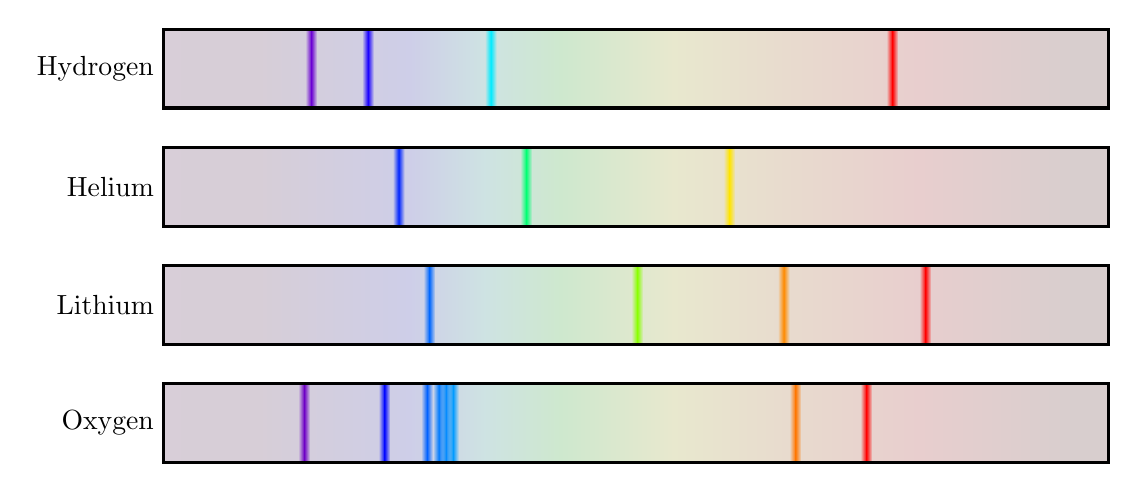
\begin{tikzpicture}[xscale=3]
	  \linespectra{0,0}{656,486,434,410}
	  \node[left] at (0,0.5) {Hydrogen};
	  \linespectra{0,-1.5}{587,501,447}
	  \node[left] at (0,-1) {Helium};
	  \linespectra{0,-3}{670,610,548,460}
	  \node[left] at (0,-2.5) {Lithium};
	  \linespectra{0,-4.5}{645,615,470,467,464,459,441,407}
	  \node[left] at (0,-4) {Oxygen};
	\end{tikzpicture}
  \end{center}
\end{frame}

\begin{frame}{Lightbulb!}
  \begin{itemize}
	\item Incandescent bulbs:
	  \begin{itemize}
		\item Hot, glowing filament
		\item Gives a black body spectra
		\item Lot of it's radiation is in the IR
	  \end{itemize}
	\item Fluorescent Lights (or vapor lamps)
	  \begin{itemize}
		\item Electrically ``excited'' gas
		\item Give a line spectra
		\item Generally more efficient
		\item May look ``unnatural''
	  \end{itemize}
  \end{itemize}
\end{frame}

\begin{frame}{Lightbulb Spectra}
  \begin{center}
	\begin{tikzpicture}
	  \clip[rounded corners] (0.2,0.5) rectangle (10.1,6.3);
	  \node[anchor=south west] at (0,0) {\includegraphics[width=10cm]{ch5_bulb_spectra.png}};
	\end{tikzpicture}
  \end{center}
\end{frame}

\begin{frame}{Absorption Spectra and Goldilocks}
  \begin{itemize}
	\item What if we have a cooler gas, but with light shining on it?
	\item Some of the radiation will be absorbed
	\item Only the ``just right'' wavelengths corresponding to the energy steps
  \end{itemize}
  \begin{center}
	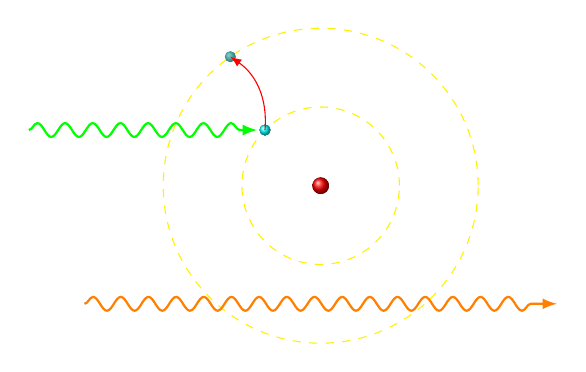
\begin{tikzpicture}
	  \coordinate (e) at (135:1);
	  \coordinate (e2) at (125:2);
	  \fill[ball color=red] (0,0) circle (3pt);
	  \draw[yellow, dashed] (0,0) circle (1cm);
	  \draw[yellow, dashed] (0,0) circle (2cm);
	  \fill[ball color=cyan] (e) circle (2pt);
	  \draw[thick,-latex, green, decorate, decoration={snake, post length=1mm}] ($(e)-(3,0)$) -- ($(e)-(1mm,0)$);
	  \fill[ball color=cyan, opacity=0.5] (e2) circle (2pt);
	  \draw[-latex, red] (e) to[bend right] (e2);
	  \draw[thick, -latex, orange, decorate, decoration={snake, post length=2mm}] (-3,-1.5) --+ (6,0);
	\end{tikzpicture}
  \end{center}
\end{frame}

\begin{frame}{Sample Case: Hydrogen}
  \begin{center}
	%\includegraphics[width=\textwidth]{ch5_emission_absorption.png}
	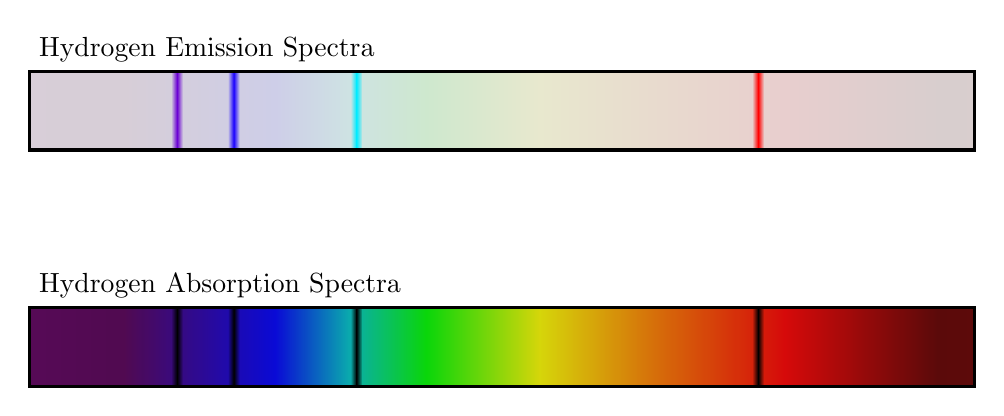
\begin{tikzpicture}[xscale=3]
	  \linespectra{0,0}{656,486,434,410}
	  \node[above right] at (0,1) {Hydrogen Emission Spectra};
	  \absorbspectra{0,-3}{656,486,434,410}
	  \node[above right] at (0,-2) {Hydrogen Absorption Spectra};
	\end{tikzpicture}
  \end{center}
\end{frame}

\begin{frame}{That Spectra is Stellar!}
  \begin{columns}
	\column{.5\textwidth}
	\begin{itemize}
	  \item You see absorption lines in spectra of stars
	  \item Stars emit a blackbody spectrum, which depends on the star's temperature
	  \item Thinner and cooler gas at the star's surface absorb some wavelengths
	\end{itemize}
	\column{.5\textwidth}
	\begin{center}
	  \includegraphics[width=\textwidth]{ch5_sun_spectrum.jpg}
	\end{center}
  \end{columns}
\end{frame}

\begin{frame}{Viewing Absorption Differently}
  \begin{center}
	\begin{tikzpicture}
	  \begin{axis}[
		  width=14cm,
		  height=7cm,
		  scaled ticks=false,
		  xlabel = Wavelength (\si{\angstrom}),
		  ylabel = Intensity,
		  xmax=8e3,
		  xmin=3.5e3,
		]
		\addplot[LBlue,thick] table[x=Wavelength, y=Flux, col sep=comma] {../Data/Ch5_starflux.txt};
	  \end{axis}
	\end{tikzpicture}
  \end{center}
\end{frame}

\begin{frame}{Recap}
  \begin{itemize}[<+->]
	\item A hot, dense source emits a continuous spectra
	\item Hot diffuse gases emit line spectra
	\item Cooler gases in front of hot sources create absorption lines
  \end{itemize}
\end{frame}

\end{document}
